\section{pH Control loop}
\subsection{Overview}
pH control is a notoriously difficult control problem not only due to its highly non-linear nature and large temperature dependence but also due to the extreme conditions experienced by measuring equipment. These problems can be investigated on the rig shown in figure~\ref{fig:rig:ph}.
\begin{figure}
	\centering
	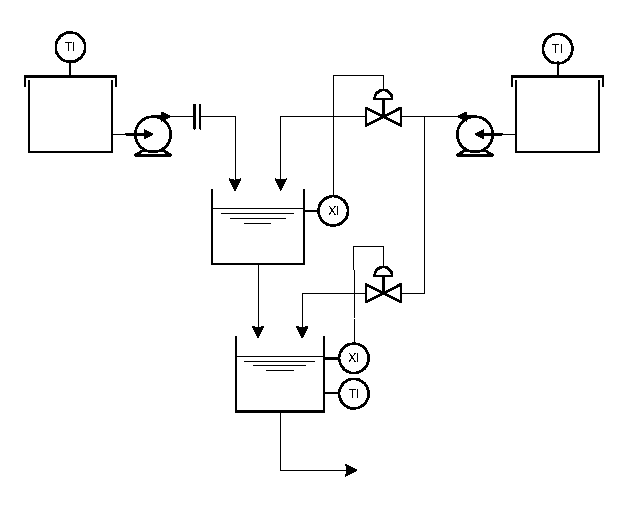
\includegraphics{pH}
	\caption{The pH control rig}
	\label{fig:rig:ph}
\end{figure}
Three temperature measurements are made to provide the possibility for temperature compensation.

\subsection{Procedures}

\subsubsection{Commissioning}

\subsubsection{Startup}

\subsubsection{Shutdown}

\subsubsection{Decommissioning}
